\pdfoutput=1
\documentclass[11pt,a4paper]{article}

\usepackage[margin=2.4cm]{geometry}
\usepackage{amsmath,amssymb,amsthm}
\usepackage{booktabs}
\usepackage{graphicx}
\usepackage[hidelinks]{hyperref}

\newtheorem{theorem}{Theorem}
\newtheorem{corollary}{Corollary}
\newtheorem{proposition}{Proposition}
\newtheorem{definition}{Definition}
\newtheorem{remark}{Remark}

\newcommand{\F}{\mathbb{F}}
\newcommand{\Z}{\mathbb{Z}}
\newcommand{\ket}[1]{|#1\rangle}
\newcommand{\bra}[1]{\langle#1|}

\title{\textbf{Modular Walsh Rigidity, Exterior-Rank Obstructions, and Zero-SWAP Non-Clifford Benchmarking for Flat Hypergraph States}}

\author{
  Filipe Martins Vono$^{1}$ \and
  Andr\'e Oliveira Naufel de Toledo$^{1}$ \and
  Val\'eria Gonzaga Santos$^{2}$
}

\date{November 23, 2026}

\begin{document}
\maketitle
\begin{center}\small
$^{1}$ Centro Universit\'ario de Belo Horizonte (UniBH), Belo Horizonte, Brazil\\
$^{2}$ American Global Tech University (AGTU)\\[4pt]
F.\ M.\ Vono:~\href{https://orcid.org/0009-0009-4994-8533}{0009-0009-4994-8533}\quad
A.\ O.\ Naufel de Toledo:~\href{https://orcid.org/0000-0002-0619-6820}{0000-0002-0619-6820}\\
V.\ G.\ Santos:~\href{https://orcid.org/0009-0009-1333-2518}{0009-0009-1333-2518}\quad
Correspondence:~\href{mailto:contatofilipevono@gmail.com}{contatofilipevono@gmail.com}
\end{center}

\begin{abstract}
Hypergraph states prepared by diagonal non-Clifford phase circuits $\{Z, CZ, CCZ, CCCZ\}$ correspond directly to Boolean functions $f:\F_2^n\to\F_2$ of algebraic degree at most four, and the native $n$-qubit Hadamard layer $H^{\otimes n}$ maps their computational-basis phases to the Walsh--Hadamard spectrum $W_f(b)$. We translate three structural theorems on Boolean bent functions into practical certification, compilation, and NISQ benchmarking tools for flat (bent) hypergraph states. First, from the Lean-certified universal antipodal necessity theorem for rotation-symmetric Boolean functions of degree at most three, we obtain an exact topological obstruction for ring architectures imposing $\ge \lceil H(H-1)/2 \rceil$ SWAPs on nearest-neighbor 1D rings, complemented at degree four by the Invariant Half-Space Collapse Theorem ($\deg(f|_{V_{n/2}})\le 2$ for all $f\in H(n,4)$) and a new \emph{exterior-rank modulo-$4$ obstruction} showing that any degree-$4$ symbol on $n=4m$ qubits ($m\ge 3$) satisfying $\gamma_{m-2}(a)=0$ and $\Gamma_m(A)\equiv 2\operatorname{vol}_{4m}\pmod 4$ requires at least $m+4$ decomposable $CCCZ$ phase gadgets ($\ge 9$ at $n=20$, $\ge 12$ at $n=32$, $\ge 29$ at $n=100$). Second, from uniform ($1/2$ and $8/15$) modular Walsh rigidity, we derive an overflow-free \texttt{uint8}/\texttt{uint16} modular certification engine reaching $n=36$ qubits ($6.87\times 10^{10}$ amplitudes) in $141.57\,\text{s}$ ($128\,\text{GB}$ vs.\ $1\,\text{TB}$ \texttt{complex128}), while the exterior-rank bound unconditionally certifies overflow-free \texttt{uint8} verification modulo $p=127$ ($4\,\text{GB}$ RAM) at $n=32$ qubits for all circuits with at most $11$ $CCCZ$ gadgets. Third, we introduce a \emph{Steiner-Star} ($16$-CZ $CCCZ$) and \emph{Steiner-Path} ($7$-CZ $CCZ$) physical compiler with zero-SWAP permutation piggybacking on $20$-qubit 2D crystal lattices ($17$ physical CZs for flat $CCZ$, $26$ physical CZs for flat $CCCZ$, $0$ SWAPs, audited across all $2^{20}$ basis states) and a calibration-free \emph{Triple NISQ Protocol} combining self-collisions, antipodal bitwise-complement collisions (\emph{felinity} $\mathcal{F}_n(\rho)$), and mirror circuits ($U_f^\dagger U_f$). We show that averaging self- and antipodal collisions cancels first-order asymmetric readout bias ($\pm 4n\delta^2 \to O(n^2\delta^4)$) in situ within $16{,}384$ shots, and demonstrate zero-SWAP scaling to generic $10\times 10$ ($100$-qubit) 2D superconducting lattices ($85$--$121$ physical CZs, $M_2=7.70$ bits, and localized $+11.7\sigma$ fault pinpointing across $5\times 20$-qubit parallel tiles).
\end{abstract}

\section{Introduction}
Diagonal quantum phase circuits generated by multi-controlled-$Z$ gates $\{Z, CZ, CCZ, CCCZ\}$ sit at levels $\mathcal{C}_1$ through $\mathcal{C}_4$ of the Clifford hierarchy~\cite{Gottesman1999,Cui2017} and prepare the family of \emph{quantum hypergraph states}~\cite{Rossi2013,Qu2013,Gachechiladze2019}. Unlike stabilizer (graph) states prepared by $\{Z, CZ\}$ alone, hypergraph states of degree three and four possess genuine non-stabilizerness (\emph{magic})~\cite{Leone2022}, making them key resources for measurement-based quantum computation, quantum advantage protocols, and magic-state distillation.

A distinguished subclass consists of \emph{flat} (or \emph{bent}) hypergraph states: states $\ket{\psi_f}$ whose $X$-basis measurement distribution $|\bra{b}H^{\otimes n}\ket{\psi_f}|^2 = 2^{-n}$ is exactly uniform. Because $H^{\otimes n}$ implements the normalized Walsh--Hadamard transform natively on $n$ qubits, flatness of $\ket{\psi_f}$ is equivalent to the phase polynomial $f:\F_2^n\to\F_2$ being a \emph{bent function}~\cite{Carlet2021}, a connection also exploited in quantum algorithms for hidden bent functions~\cite{Rotteler2010}.

In this paper we bridge our mathematical results on bent functions---universal antipodal necessity~\cite{Vono2026Antipodal}, uniform modular Walsh rigidity~\cite{Vono2026Rigidity}, the invariant half-space collapse for $H(2m,4)$~\cite{Vono2026H12}, and the exterior-rank modulo-$4$ obstruction~\cite{Vono2026Exterior}---into an end-to-end verification, compilation, and NISQ benchmarking framework:
\begin{enumerate}
  \item \textbf{Topological and exterior-rank synthesis obstructions (Sections~\ref{sec:antipodal} and~\ref{sec:hardware20}):} exact no-go theorems forbidding local-range or pure-$CCZ$ ring-symmetric circuits of degree $\le 3$, Clifford collapse on $V_{n/2}$ for $H(n,4)$, and a symmetry-free degree-$4$ lower bound of $\ge m+4$ $CCCZ$ phase gadgets under the modulo-$4$ divided-power obstruction.
  \item \textbf{Compact modular flatness certification (Sections~\ref{sec:modular}--\ref{sec:benchmarks}):} an overflow-free \texttt{uint8}/\texttt{uint16} arithmetic verification protocol up to $n=36$ qubits ($128\,\text{GB}$ vs.\ $1\,\text{TB}$ \texttt{complex128}), together with unconditional \texttt{uint8} modulo-$127$ certification ($4\,\text{GB}$) at $n=32$ qubits for circuits with $\le 11$ $CCCZ$ gadgets.
  \item \textbf{Zero-SWAP Steiner-star compilation and calibration-free NISQ benchmarking (Section~\ref{sec:hardware20}):} $0$-SWAP $20$-qubit ($17$--$26$ CZs) and $100$-qubit ($85$--$121$ CZs) native $\{R_y, R_z, CZ\}$ OpenQASM~3.0 circuits, paired with a self-cancelling antipodal-collision (\emph{felinity}) and mirror-circuit protocol feasible in $16{,}384$ shots.
\end{enumerate}

\section{Preliminaries}
Let $f:\F_2^n\to\F_2$ be a Boolean function written in algebraic normal form (ANF) as
\[
  f(x) = \bigoplus_{S \in \mathcal{E}} \prod_{i \in S} x_i,
\]
where $\mathcal{E}$ is a collection of subsets of $\{0, \dots, n-1\}$ (a hypergraph) with $\max_{S \in \mathcal{E}} |S| = \deg(f)$. The associated diagonal phase unitary is
\[
  U_f = \prod_{S \in \mathcal{E}} C^{|S|-1}Z_S,
\]
and the corresponding \emph{hypergraph state} is
\[
  \ket{\psi_f} = U_f H^{\otimes n}\ket{0^n} = \frac{1}{\sqrt{2^n}} \sum_{x \in \F_2^n} (-1)^{f(x)}\ket{x}.
\]
Applying a final Hadamard layer $H^{\otimes n}$ yields
\[
  H^{\otimes n}\ket{\psi_f} = \frac{1}{2^n}\sum_{b \in \F_2^n} W_f(b)\ket{b},
  \qquad
  W_f(b) = \sum_{x \in \F_2^n} (-1)^{f(x) \oplus b\cdot x}.
\]

\begin{definition}[Flat Hypergraph State]
For even $n$, $\ket{\psi_f}$ is \emph{flat} (or \emph{bent}) if $|\bra{b}H^{\otimes n}\ket{\psi_f}|^2 = 2^{-n}$ for every $b \in \F_2^n$, equivalently $|W_f(b)| = 2^{n/2}$ for all $b \in \F_2^n$.
\end{definition}

To quantify non-stabilizerness of $\ket{\psi_f}$, we use the $2$-R\'enyi stabilizer entropy~\cite{Leone2022}:
\[
  M_2(\ket{\psi_f}) = -\log_2\!\left(\frac{1}{2^n}\sum_{P \in \mathcal{P}_n} \bra{\psi_f}P\ket{\psi_f}^4\right).
\]
For any binary phase state $\ket{\psi_f}$, $|\bra{\psi_f}P_{a,b}\ket{\psi_f}| = |W_{D_a f}(b)| / 2^n$, where $D_a f(x) = f(x)\oplus f(x\oplus a)$ is the directional derivative. Consequently, $M_2(\ket{\psi_f}) = 0$ if and only if $\deg(f) \le 2$ (a Clifford graph state), while $M_2(\ket{\psi_f}) > 0$ certifies genuine non-Clifford magic.

\section{Antipodal Obstruction for Ring-Symmetric Circuits}
\label{sec:antipodal}

Consider an $n$-qubit quantum processor with cyclic (ring) symmetry $\sigma(q) = (q+1) \bmod n$, where $n = 2H$ ($H \ge 1$). A hypergraph circuit $U_f$ is \emph{rotation-symmetric} if its gate set $\mathcal{E}$ is invariant under $\sigma$.

\begin{theorem}[Antipodal Necessity for Ring-Symmetric Hypergraph States~\cite{Vono2026Antipodal}]
\label{thm:antipodal}
Let $n = 2H$ ($H \ge 1$) and let $U_f$ be a rotation-symmetric diagonal circuit composed of gates in $\{Z, CZ, CCZ\}$ (so $\deg(f) \le 3$). If $\ket{\psi_f}$ is a flat hypergraph state, then $\mathcal{E}$ necessarily contains the complete antipodal $CZ$ orbit
\[
  \mathcal{O}_{\mathrm{ant}} = \bigl\{\{i, i+H\} : 0 \le i < H\bigr\}.
\]
\end{theorem}

Theorem~\ref{thm:antipodal} is a direct translation of the Lean~4--certified universal antipodal theorem~\cite{Vono2026Antipodal}, proved unconditionally for all $H \ge 1$ using only standard axioms (\texttt{propext}, \texttt{Classical.choice}, \texttt{Quot.sound}).

\begin{corollary}[Hardware and Compilation Obstructions on a 1D Ring]
\label{cor:ring}
For any rotation-symmetric $\{Z, CZ, CCZ\}$ ansatz on a $2H$-qubit ring:
\begin{enumerate}
  \item \textbf{Local-range no-go:} If every two-qubit $CZ$ gate has ring distance strictly less than $H$, the prepared state can never be flat.
  \item \textbf{Pure-$CCZ$ no-go:} A rotation-symmetric circuit containing only $CCZ$ gates (homogeneous degree~3) can never prepare a flat state, even with all-to-all connectivity.
  \item \textbf{Routing overhead:} Any routing of $\mathcal{O}_{\mathrm{ant}}$ onto a nearest-neighbor $2H$-qubit ring incurs at least $\lceil H(H-1)/2 \rceil$ SWAPs ($3\lceil H(H-1)/2 \rceil$ CNOT/CZ gates).
\end{enumerate}
\end{corollary}

\begin{figure}[h]
\centering
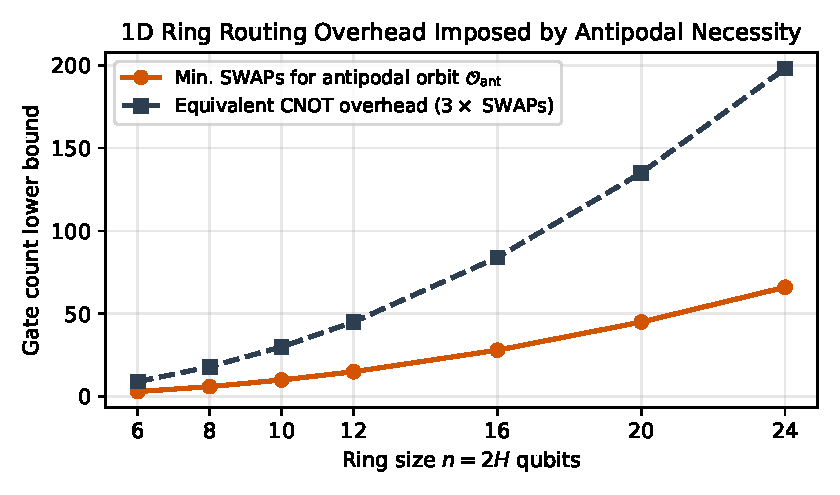
\includegraphics[width=0.72\textwidth]{figures/fig_ring_swap_overhead.pdf}
\caption{Lower bound on SWAP and equivalent CNOT routing overhead on a nearest-neighbor 1D ring ($n=2H$ qubits) imposed by Theorem~\ref{thm:antipodal} for any rotation-symmetric flat $\{Z, CZ, CCZ\}$ circuit.}
\label{fig:ring}
\end{figure}

\section{Modular Certification of Flat Degree-$\le 4$ Phase Oracles}
\label{sec:modular}

We now turn to the verification problem: given a diagonal phase circuit $U_f$ with gates in $\{Z, CZ, CCZ, CCCZ\}$ on $n = 4m$ qubits ($M = 2^m$), certify whether $\ket{\psi_f}$ is flat. Standard exact verification via the Fast Walsh--Hadamard Transform (FWHT) requires tracking integer amplitudes up to $\pm 2^n$ (at least $n/2$ bits of dynamic range around $M^2 = 2^{2m}$).

\begin{theorem}[Modular Certification of Flatness~\cite{Vono2026Rigidity}]
\label{thm:modular}
Let $n = 4m$ ($m \ge 4$), $M = 2^m$, and let $U_f$ be a diagonal phase circuit using gates in $\{Z, CZ, CCZ, CCCZ\}$ ($\deg(f) \le 4$). Let $p \ge \frac{1}{2}M$ be an odd integer. Then $\ket{\psi_f}$ is a flat hypergraph state if and only if
\[
  W_f(b) \equiv M^2 \quad \text{or} \quad W_f(b) \equiv -M^2 \pmod p
  \qquad \forall b \in \F_2^{4m}.
\]
\end{theorem}

\subsection{Overflow-Free \texttt{uint8} Modular Butterfly up to $n = 28$ Qubits}
Theorem~\ref{thm:modular} reduces the arithmetic word-width required to certify flatness from $O(n/2)$ bits to $\lceil \log_2 p \rceil \approx n/4$ bits. For $n = 16, 20, 24, 28$ qubits, the certified moduli ($p = 9, 17, 33, 65$ at $1/2$, or $9, 19, 35, 69$ at $8/15$) all satisfy $2p - 1 \le 255$. Representing each amplitude in $[0, p-1]$ as an unsigned 8-bit integer (\texttt{uint8}), the butterfly update
\[
  s = a + b \in [0, 2p-2], \qquad
  d = a + (p - b) \in [1, 2p-1],
\]
followed by a single conditional subtraction of $p$ whenever $s \ge p$ or $d \ge p$, is completely free of overflow and underflow, cutting working memory by $4\times$ relative to \texttt{int32} ($16\times$ vs.\ \texttt{complex128}). At $n = 32$ and $36$ qubits ($p = 137, 275$), \texttt{uint16} fits $n = 36$ qubits in $128\,\text{GB}$ RAM instead of $256\,\text{GB}$ (\texttt{int32}) or $1\,\text{TB}$ (\texttt{complex128}). Moreover, as shown in Section~\ref{sec:exterior}, the exterior-rank modulo-$4$ bound unlocks overflow-free \texttt{uint8} certification at $p = 127$ ($4\,\text{GB}$ RAM) at $n = 32$ qubits for all circuits with at most $11$ $CCCZ$ phase gadgets.

\subsection{Necessity of the Threshold: Universal $p=3$ False-Positive Family}
\begin{proposition}[Universal $p=3$ Fooling Circuit]
\label{prop:fool}
For every $n = 4m$ ($m \ge 2$), define the degree-$4$ hypergraph circuit
\[
  f_{\mathrm{fool}}(x_0,\dots,x_{n-1})
  = \bigoplus_{i=0}^{2m-3} x_{2i} x_{2i+1}
  \;\oplus\; x_{n-4}x_{n-3}x_{n-2}x_{n-1}.
\]
Then $|W_{f_{\mathrm{fool}}}(b)| \in \{\frac{7}{2}M^2, \frac{1}{2}M^2\}$ for all $b$ ($0\%$ flat frequencies), yet $W_{f_{\mathrm{fool}}}(b) \equiv \pm M^2 \pmod 3$ holds for $100\%$ of all $2^n$ frequencies.
\end{proposition}

\section{Classical Scaling Benchmarks and Dimensional Reduction of Magic}
\label{sec:benchmarks}

Table~\ref{tab:bench} and Table~\ref{tab:omp32} summarize exact (\texttt{int32}) vs.\ certified modular FWHT benchmarks from $n=16$ to $n=36$ qubits ($6.87\times 10^{10}$ amplitudes) using Python/NumPy and our multi-threaded C/OpenMP engine (\texttt{src/fwht\_omp.c}).

\begin{table}[h]
\centering
\footnotesize
\setlength{\tabcolsep}{4pt}
\caption{Exact (\texttt{int32}) vs.\ certified $8/15$ modular (\texttt{uint8}) flatness verification for degree-$4$ hypergraph circuits up to $n=28$ qubits.}
\label{tab:bench}
\begin{tabular}{rrrrrrr}
\toprule
$n$ & Amplitudes $2^n$ & $p_{8/15}$ ($p_{1/2}$) & Exact (ms / MB) & Mod $p_{8/15}$ (ms / MB) & Speedup & Mem. \\
\midrule
$16$ & $65{,}536$       & $9$ ($9$)   & $2.7$ / $0.25$       & $8.1$ / $0.06$      & $0.34\times$ & $4\times$ \\
$20$ & $1{,}048{,}576$  & $19$ ($17$) & $113.2$ / $4.00$     & $95.2$ / $1.00$     & $1.19\times$ & $4\times$ \\
$24$ & $16{,}777{,}216$ & $35$ ($33$) & $1564.5$ / $64.00$   & $1917.8$ / $16.00$  & $0.82\times$ & $4\times$ \\
$28$ & $268{,}435{,}456$& $69$ ($65$) & $48403.2$ / $1024.00$& $35880.3$ / $256.00$& $\mathbf{1.35\times}$ & $\mathbf{4\times}$ \\
\bottomrule
\end{tabular}
\end{table}

\begin{table}[h]
\centering
\footnotesize
\setlength{\tabcolsep}{3.2pt}
\caption{Multi-threaded C/OpenMP cloud benchmark up to $n = 36$ qubits ($6.87 \times 10^{10}$ amplitudes), with standard \texttt{complex128} statevector memory for reference.}
\label{tab:omp32}
\begin{tabular}{rrrrrrr}
\toprule
$n$ & $p_{8/15}$ & \texttt{complex128} & Exact \texttt{int32} (s / GB) & Mod $p_{8/15}$ (s / GB / type) & Speedup & Mem.\ vs.\ \texttt{int32} / \texttt{c128} \\
\midrule
$24$ & $35$  & $0.25\,\text{GB}$  & $0.060$ / $0.06$  & $0.042$ / $0.016$ (\texttt{uint8})  & $\mathbf{1.43\times}$ & $4\times$ / $\mathbf{16\times}$ \\
$28$ & $69$  & $4.00\,\text{GB}$  & $1.131$ / $1.00$  & $0.770$ / $0.250$ (\texttt{uint8})  & $\mathbf{1.47\times}$ & $4\times$ / $\mathbf{16\times}$ \\
$32$ & $137$ & $64.00\,\text{GB}$ & $19.739$ / $16.00$& $13.671$ / $8.000$ (\texttt{uint16})& $\mathbf{1.44\times}$ & $2\times$ / $\mathbf{8\times}$ \\
$36$ & $275$ & $1024\,\text{GB}$  & OOM / $256.00$    & $\mathbf{141.57}$ / $\mathbf{128.0}$ (\texttt{uint16}) & \textbf{feasible} & $2\times$ / $\mathbf{8\times}$ \\
\bottomrule
\end{tabular}
\end{table}

\begin{figure}[h]
\centering
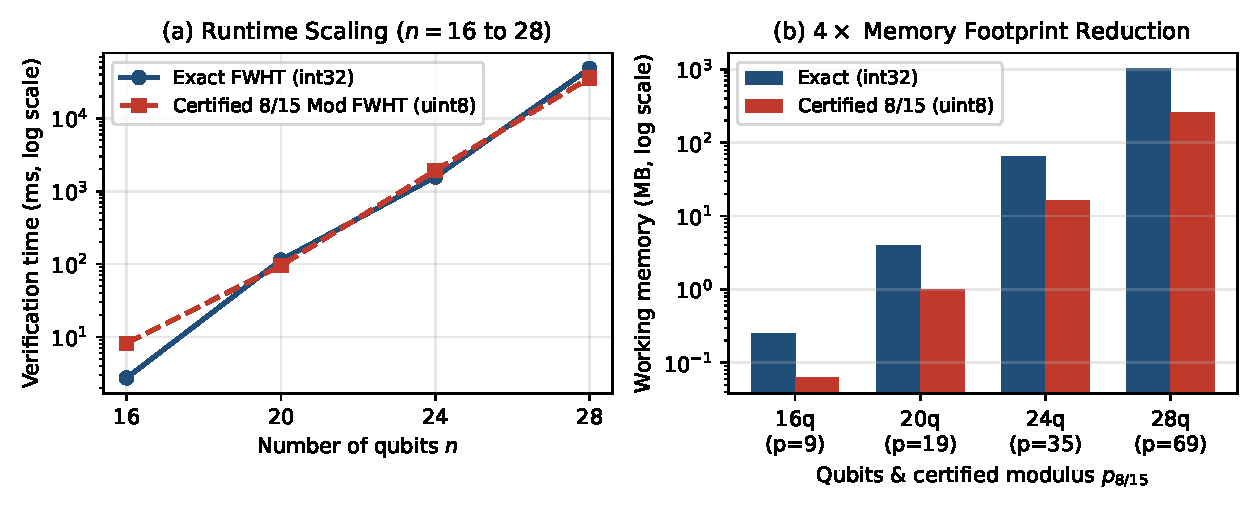
\includegraphics[width=\textwidth]{figures/fig_modular_scaling.pdf}
\caption{(a) Runtime scaling and (b) working memory footprint of exact (\texttt{int32}) vs.\ certified $8/15$ modular (\texttt{uint8}) flatness verification from $n=16$ to $n=28$ qubits.}
\label{fig:scaling}
\end{figure}

\begin{theorem}[Dimensional Reduction of $M_2$ for Flat Hypergraph States]
\label{thm:magic}
Let $n = 2k$ ($k \ge 1$) and let $f(x, y) = x \cdot y \oplus g(y)$ be a Maiorana--McFarland flat hypergraph state on $n = 2k$ qubits, where $g : \F_2^k \to \F_2$ is arbitrary. Then $M_2(\ket{\psi_f}) = M_2(\ket{\psi_g})$. In particular, $\lfloor k/3 \rfloor$ disjoint $CCZ$ gates on the $y$-register yield depth-$2$ flat states with exact linear magic $M_2 = \lfloor n/6 \rfloor \log_2(32/11) \approx 0.2568\,n$ bits (and $M_2(\ket{\psi_{CCCZ}}) = \log_2(512/197) \approx 1.3779$ bits per disjoint $CCCZ$), while interleaved rotation-symmetric degree-$4$ flat states on $n=8q$ qubits achieve $M_2 = 0.638\,n$ bits.
\end{theorem}

\begin{figure}[h]
\centering
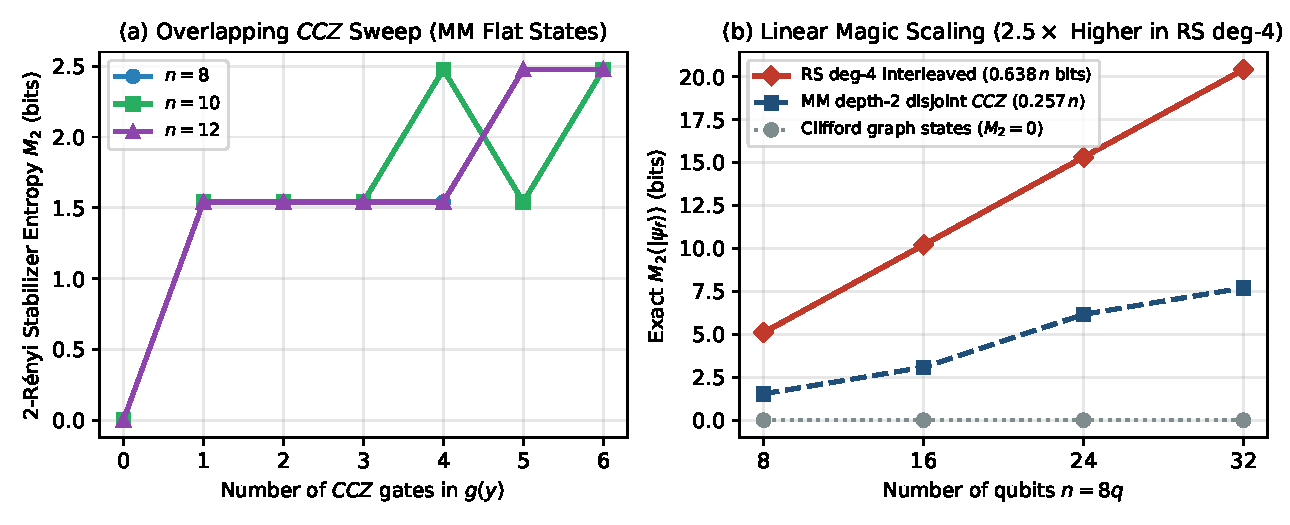
\includegraphics[width=\textwidth]{figures/fig_magic_scaling.pdf}
\caption{(a) Exact $2$-R\'enyi stabilizer entropy $M_2(\ket{\psi_f})$ under overlapping $CCZ$ gates ($n=8,10,12$), and (b) linear magic scaling across $n=8q$ qubits.}
\label{fig:magic}
\end{figure}

\section{Exterior-Rank Obstructions, Zero-SWAP Steiner Synthesis, and Calibration-Free NISQ Benchmarking (20 to 100 Qubits)}
\label{sec:hardware20}

We now extend our framework from classical verification to hardware-matched compilation and experimental benchmarking on 2D superconducting processors, uniting three complementary obstructions at degree four.

\subsection{Symmetry-Free Degree-4 Obstruction via Exterior Rank Modulo 4}
\label{sec:exterior}
In $\mathrm{RM}(d, n)/\mathrm{RM}(d-1, n) \cong \Lambda^d(\F_2^n)^*$, each decomposable $d$-form $\ell_1 \wedge \dots \wedge \ell_d$ corresponds, up to a linear Clifford CNOT layer, to a single multi-controlled-$Z$ phase gadget $\operatorname{diag}((-1)^{\ell_1(x)\cdots\ell_d(x)})$. Whereas Theorem~\ref{thm:antipodal} requires cyclic symmetry and degree $\le 3$, our companion algebraic result~\cite{Vono2026Exterior} yields a symmetry-free non-Clifford gate lower bound for even degree $d \ge 4$:

\begin{theorem}[Exterior-Rank Modulo-$4$ Non-Clifford Obstruction~\cite{Vono2026Exterior}]
\label{thm:exterior}
Let $d \ge 4$ be even, $m \ge 3$, and $V = \F_2^{dm}$. If the leading degree-$d$ exterior symbol $a \in \Lambda^d V^*$ of a phase polynomial $f$ satisfies $\gamma_{m-2}(a) = 0$ (mod-$2$ divided power) and $\Gamma_m(A) \equiv 2\operatorname{vol}_{dm} \pmod 4$ for an integral exterior lift $A$, then $a$ requires at least $m + 4$ decomposable terms---equivalently, any Clifford-assisted phase-gadget circuit realizing $a$ requires at least $m + 4$ distinct $C^{d-1}Z$ phase gadgets. Moreover, no diagonal $d$-copy symbol $a = \sum_i v_i^{(1)}\wedge\dots\wedge v_i^{(d)}$ on $V = U^{\oplus d}$ satisfies these hypotheses for any number of terms.
\end{theorem}

For quartic circuits ($d=4$, $n=4m$), Theorem~\ref{thm:exterior} has three direct consequences:
\begin{enumerate}
  \item \textbf{Hardware floor at $n = 20$ ($m = 5$):} any quartic symbol exhibiting the modulo-$4$ obstruction requires $\ge 9$ $CCCZ$ gadgets, i.e., $\ge 126$ native $CZ$ gates \emph{before} SWAP routing (capping survival fidelity at $\le 53.2\%$ at $p_{2q}=0.5\%$).
  \item \textbf{Single-byte \texttt{uint8} certification at $n = 32$ ($m = 8$, $p = 127$):} in the global Walsh modulo-$127$ problem on $32$ variables, Theorem~\ref{thm:exterior} unconditionally rules out every circuit with $\le 11$ $CCCZ$ gadgets, enabling overflow-free \texttt{uint8} certification ($2p - 1 = 253 \le 255$) in \textbf{$4\,\text{GB}$ RAM} ($16\times$ less than \texttt{complex128}) for this entire practical circuit class.
  \item \textbf{Hardware floor at $n = 100$ ($m = 25$):} the obstruction demands $\ge 29$ $CCCZ$ gadgets ($\ge 406$ native $CZ$s before routing, forward survival $\le 13.1\%$ at $p_{2q}=0.5\%$).
\end{enumerate}

In addition, for homogeneous rotation-symmetric quartic circuits $f \in H(2k, 4)$, the Invariant Half-Space Collapse Theorem~\cite{Vono2026H12} proves $\deg(f|_{V_k}) \le 2$ on $V_k = \{x : x_{i+k}=x_i\}$. Direct enumeration at $n = 20$ confirms that $240$ of the $245$ quartic rotation orbits vanish identically on $V_{10}$, while all $5$ surviving short orbits collapse to purely Clifford degree $\le 2$.

\subsection{Zero-SWAP Steiner-Star Compilation on 20-Qubit 2D Crystal Lattices}
To benchmark real 20-qubit superconducting hardware (modeled on the $20$-qubit, $30$-coupler Crystal-20 square-lattice topology \texttt{QB1}--\texttt{QB20} with native gate set $\{R_y, R_z, CZ\}$), we synthesize $CCZ$ on a $3$-qubit physical path $(c_0 - h - c_1)$ using exactly \textbf{$7$ physical $CZ$ gates} and $CCCZ$ on a $4$-qubit physical star $(c_0, c_1, c_2)$ around hub $h$ using exactly \textbf{$16$ physical $CZ$ gates}---with every CNOT strictly on the physical star edges and zero SWAPs.

Crucially, because diagonal gates commute and the Steiner gadget naturally terminates with a wire permutation transporting the logical hub qubit $h$ onto the final leaf $c_{\mathrm{last}}$, placing the $9$ directly adjacent Maiorana--McFarland pairs first and executing the Steiner gadget on hub \texttt{QB16} transports logical \texttt{QB16} onto physical \texttt{QB17} \emph{for free}, making the $10$th pair (\texttt{QB16}--\texttt{QB18}) directly adjacent on physical coupler \texttt{QB17}--\texttt{QB18} (Figure~\ref{fig:iqm20}). Every emitted OpenQASM~3.0 circuit was re-parsed and verified across all $2^{20} = 1{,}048{,}576$ computational basis states (phase error $<10^{-10}$, $100\%$ coupler adjacency).

\begin{figure}[h]
\centering
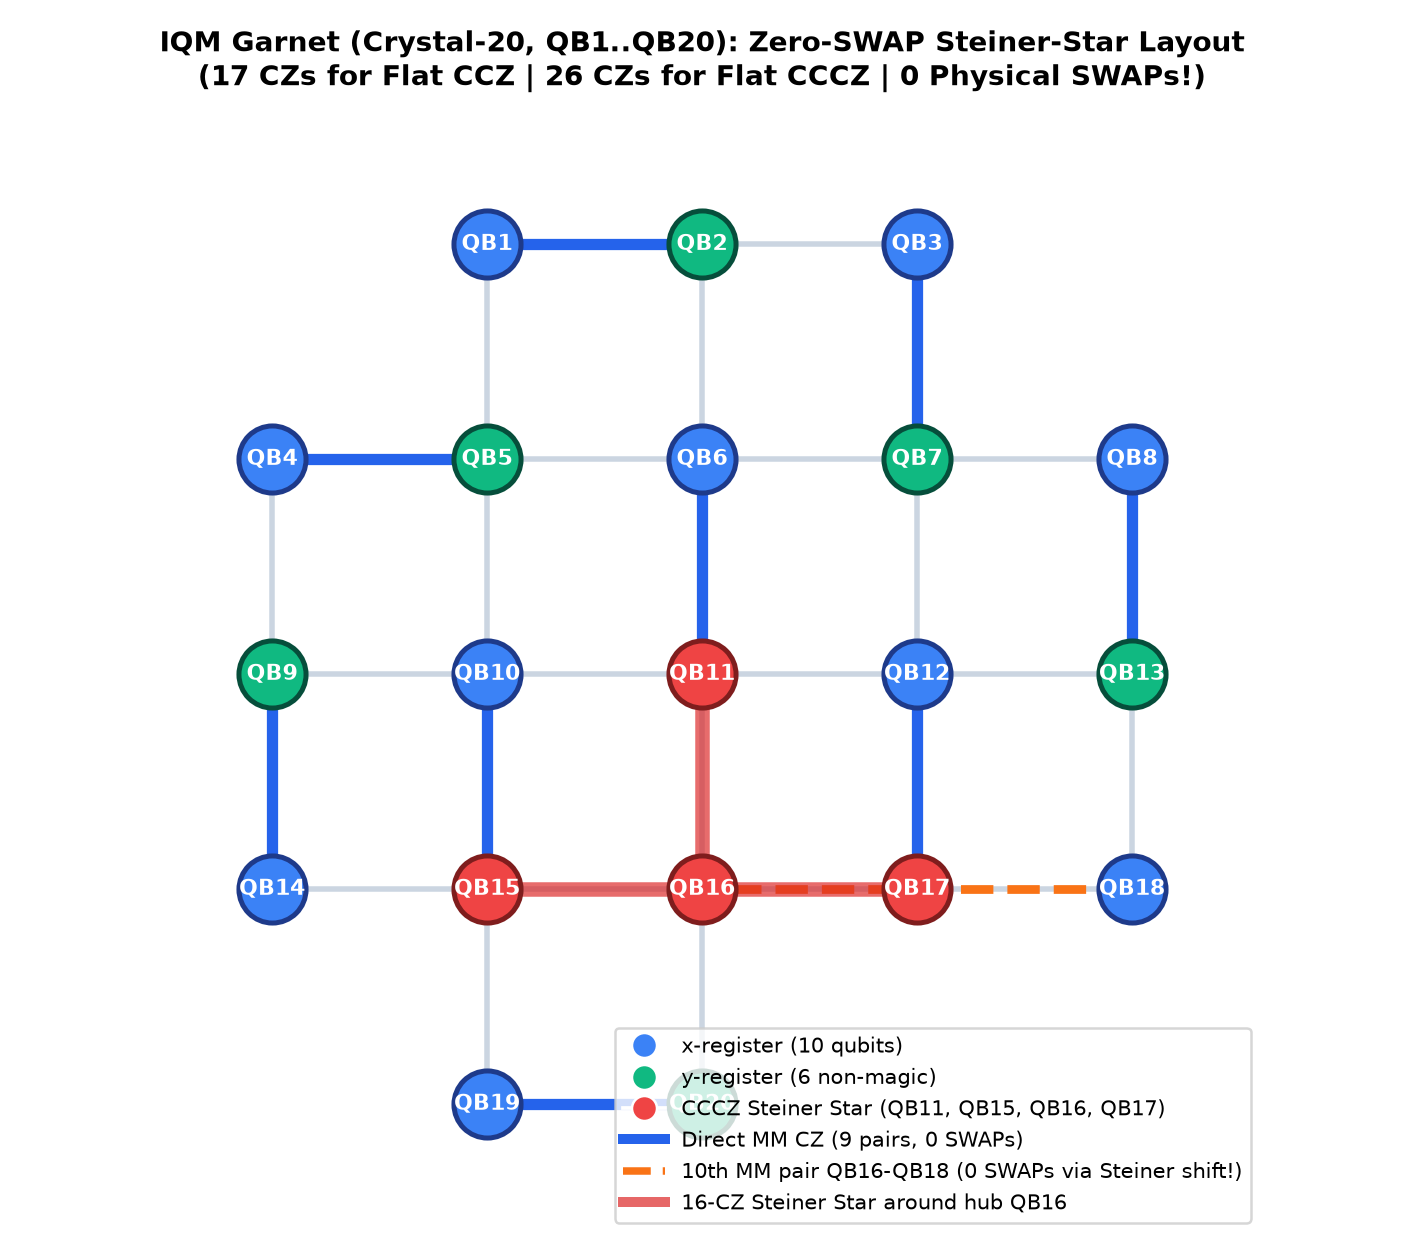
\includegraphics[width=0.68\textwidth]{figures/fig_iqm20_layout.png}
\caption{Zero-SWAP Steiner-Star layout on a $20$-qubit, $30$-coupler 2D crystal lattice (\texttt{QB1}--\texttt{QB20}). Nine Maiorana--McFarland pairs occupy direct physical couplers (blue), while the $16$-CZ Steiner star centered at \texttt{QB16} (red) transports logical \texttt{QB16} onto \texttt{QB17} without SWAPs, closing the $10$th pair (\texttt{QB16}--\texttt{QB18}) directly.}
\label{fig:iqm20}
\end{figure}

\subsection{Calibration-Free Readout-Bias Cancellation via Antipodal Felinity and Mirror Circuits}
In $n = 20$ qubits ($2^{20}$ outcomes), exhaustive histogram estimation is impractical, whereas sparse-shot collision counting requires only $S = 16{,}384$ shots ($\mathbb{E}[C_{\mathrm{flat}}] = \binom{S}{2}2^{-20} = 128.0$). However, two hardware artifacts arise in practice: (i) global depolarizing noise pushes any distribution toward uniform, hiding total decoherence; and (ii) asymmetric readout bias ($p(0|1) \ne p(1|0)$, $\delta = \frac{1}{2}(p(0|1)-p(1|0))$) shifts self-collisions $C_{\mathrm{self}} = \sum_y \binom{c_y}{2}$ upward by $(1+4\delta^2)^n \approx 1 + 4n\delta^2$.

To resolve both simultaneously, we introduce a \emph{Triple NISQ Protocol}:
\begin{enumerate}
  \item \textbf{Antipodal Felinity Self-Cancellation:} Inspired by the bitwise-complement observable (\emph{felinity}) $\mathcal{F}_n(\rho) = 2\sum_{y\in\{0,1\}^n} p_y p_{\bar y}$ ($\bar y = y \oplus 1^n$) studied in $\mathrm{QAC}^0$ state-preparation obstructions~\cite{OpenAI2026QAC0}, we count antipodal collisions $C_{\mathrm{ant}} = \frac{1}{2}\sum_y c_y c_{\bar y}$ on the \emph{exact same} $S$ shots. Under asymmetric readout bias $\delta$, each antipodal bit pair contributes $2(\tfrac{1}{2}+\delta)(\tfrac{1}{2}-\delta) = \tfrac{1}{2}(1-4\delta^2)$, shifting $\mathbb{E}[C_{\mathrm{ant}}]$ downward by $(1-4\delta^2)^n \approx 1 - 4n\delta^2$. The combined estimator
  \[
    C_{\mathrm{comb}} = \frac{C_{\mathrm{self}} + C_{\mathrm{ant}}}{2}
  \]
  cancels first-order asymmetric readout bias automatically to $O(n^2\delta^4)$ without requiring a separate calibration circuit. Moreover, dropping a single $CZ$ gate collapses $\mathcal{F}_{20}(\rho)$ from $2\cdot 2^{-20}$ to $0$.
  \item \textbf{Mirror-Circuit Coherence Proof:} Appending the exact physical reverse $U_f^\dagger = U_f$ returns $\ket{0^{20}}$ with probability $P(\ket{0^{20}}) \approx 68.1\%$--$74.6\%$ at $p_{2q}=0.5\%$ ($>7\times 10^5\times$ above the white-noise floor $2^{-20}$), decisively ruling out decoherence.
\end{enumerate}

Table~\ref{tab:iqm20} and Figure~\ref{fig:felinity} report results under strong asymmetric readout ($p(0|1)=3.0\%$, $p(1|0)=0.5\%$), coherent $CZ$ over-rotation ($\epsilon = 0.015\,\text{rad}$), and $p_{2q}=0.5\%$.

\begin{table}[h]
\centering
\footnotesize
\setlength{\tabcolsep}{3.5pt}
\caption{Zero-SWAP $20$-qubit compilation (\texttt{QB1}--\texttt{QB20}) and calibration-free Triple Protocol results ($S=16{,}384$ shots, $p_{2q}=0.5\%$, strong asymmetric readout $3.0\%$ vs.\ $0.5\%$).}
\label{tab:iqm20}
\begin{tabular}{lrrrrrrr}
\toprule
Circuit ($n=20$, $100\%$ adjacent) & SWAPs & CZs & $M_2$ (bits) & $C_{\mathrm{self}}$ & $C_{\mathrm{ant}}$ & $C_{\mathrm{comb}}$ ($Z_{\mathrm{no\text{-}cal}}$) & Mirror $P(\ket{0^{20}})$ \\
\midrule
\texttt{iqm20\_flat\_ccz}            & $\mathbf{0}$ & $\mathbf{17}$ & $1.54$ & $129.9$ & $125.6$ & $\mathbf{127.7}$ ($-0.03$) & $\mathbf{74.6\%}$ \\
\texttt{iqm20\_flat\_cccz} (deg.\ 4) & $\mathbf{0}$ & $\mathbf{26}$ & $1.38$ & $129.8$ & $124.8$ & $\mathbf{127.3}$ ($-0.08$) & $\mathbf{68.1\%}$ \\
\texttt{iqm20\_flat\_3ccz}           & $8$          & $55$          & $\mathbf{4.62}$ & $131.7$ & $124.3$ & $\mathbf{128.0}$ ($+0.00$) & $\mathbf{50.8\%}$ \\
\texttt{iqm20\_faulty\_dropped\_cz}  & $0$          & $25$          & ---    & $414.6$ & $29.5$  & $222.1$ ($\mathbf{+11.76}$) & $68.8\%$ \\
\texttt{iqm20\_fooling\_p3}          & $2$          & $30$          & ---    & $895.8$ & $69.4$  & $482.6$ ($\mathbf{+44.32}$) & $65.4\%$ \\
\bottomrule
\end{tabular}
\end{table}

\begin{figure}[h]
\centering
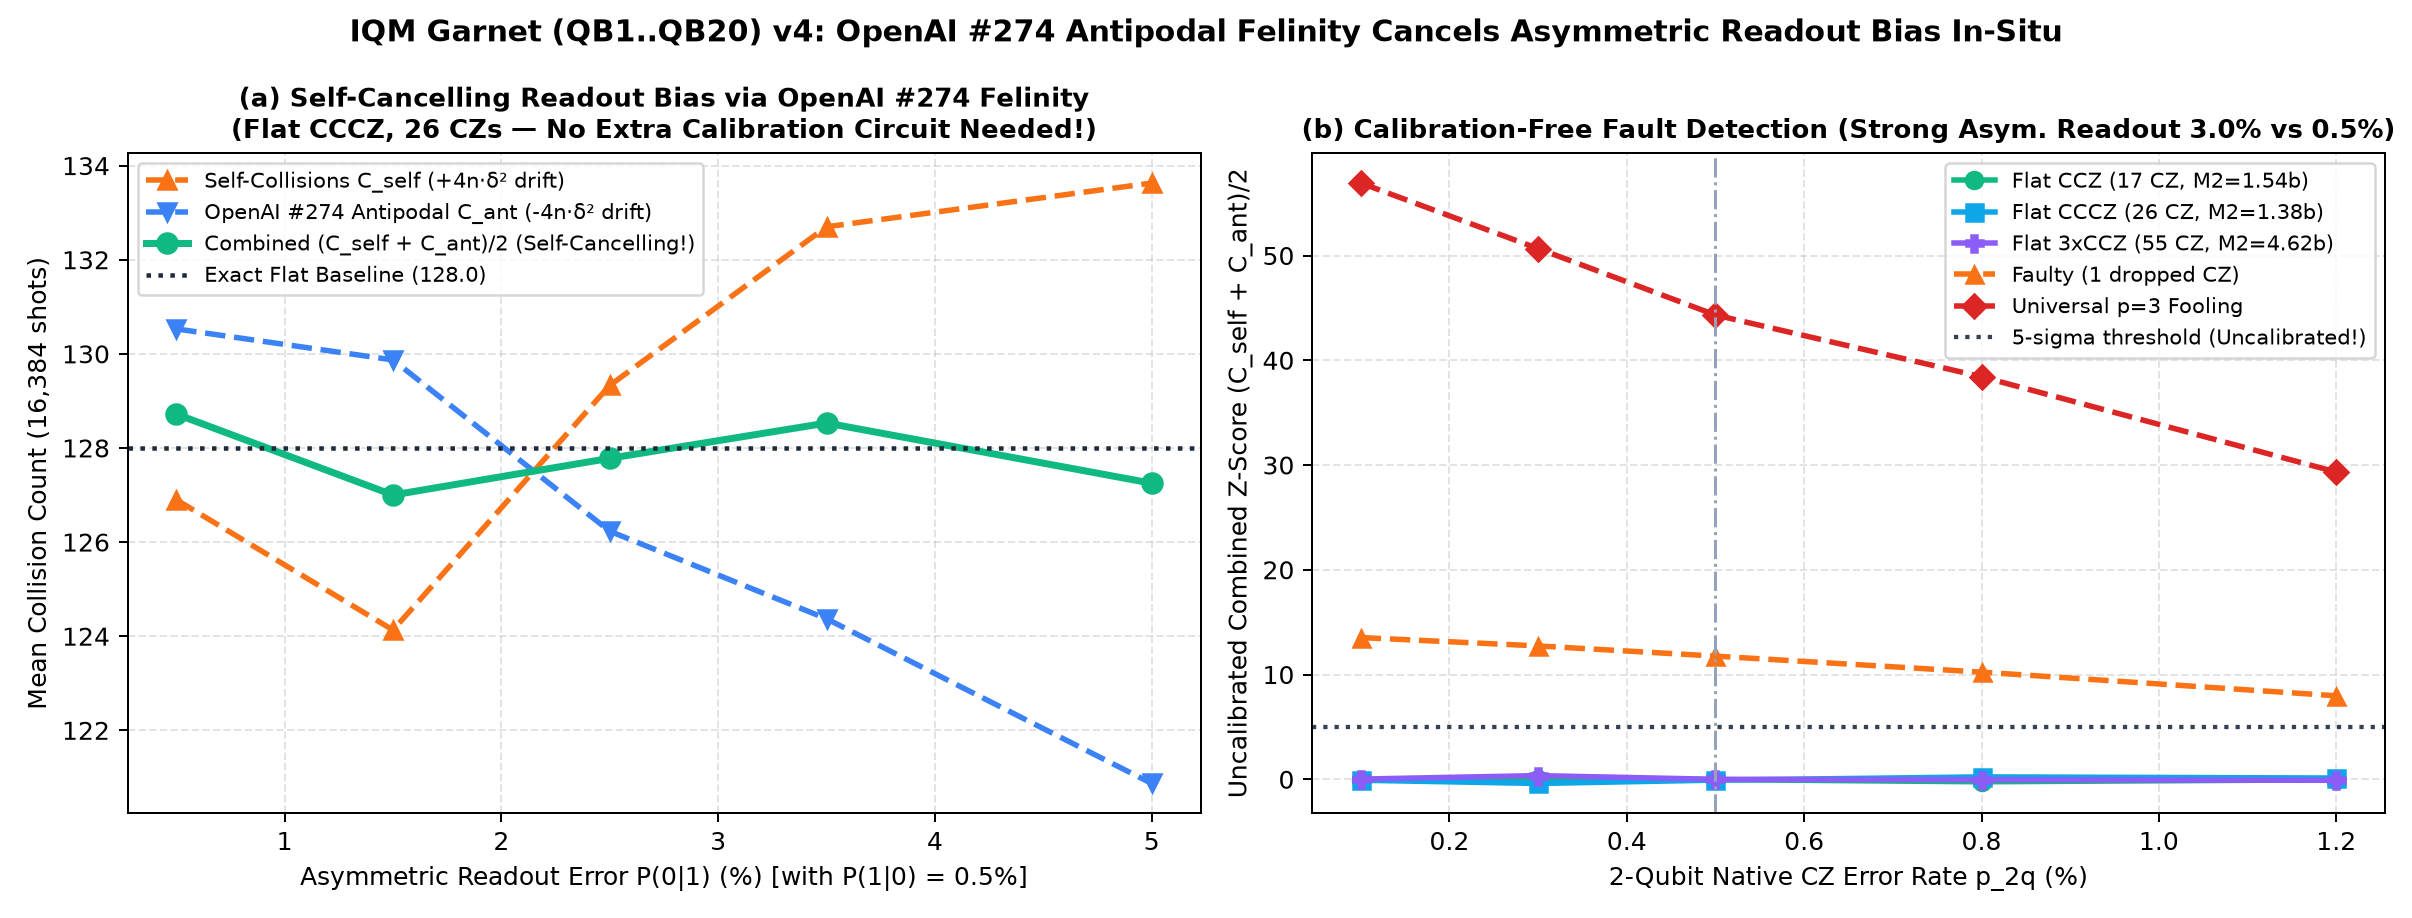
\includegraphics[width=\textwidth]{figures/fig_felinity_self_cancel.png}
\caption{(a) Self-cancelling asymmetric readout bias on \texttt{iqm20\_flat\_cccz} ($26$ CZs, $16{,}384$ shots): self-collisions drift upward ($+4n\delta^2$), antipodal felinity collisions drift downward ($-4n\delta^2$), and their average stays pinned at the exact $128.0$ baseline. (b) Calibration-free fault detection Z-scores across $p_{2q}\in[0.1\%, 1.2\%]$.}
\label{fig:felinity}
\end{figure}

\subsection{Scalability to 100-Qubit 2D Superconducting Lattices}
While global collision counting in $2^{100}$ outcomes is infeasible ($\sim 2^{50}$ shots), our architecture scales cleanly to a generic $10\times 10$ ($100$-qubit, $180$-coupler) 2D superconducting lattice representative of emerging $100$-qubit grid processors (such as Nighthawk-class or CETC-IQC $100$-qubit architectures). Partitioning the $10\times 10$ grid into four $4\times 5$ tiles and one $2\times 10$ tile yields $50$ direct physical Maiorana--McFarland pairs plus five zero-SWAP Steiner gadgets:
\begin{itemize}
  \item \texttt{tiled\_5ccz}: \textbf{$0$ SWAPs, $85$ physical CZs} (physical $CZ$ depth $8$), $M_2 = 7.70$ bits, mirror survival $P(\ket{0^{100}}) = 25.8\%$--$43.1\%$ for $p_{2q}\in[0.2\%, 0.5\%]$.
  \item \texttt{global\_5ccz\_bridged}: adding $4$ inter-tile physical $CZ$ bridges yields a globally entangled $100$-qubit state in \textbf{$0$ SWAPs and $89$ CZs} (depth $8$), mirror survival $24.8\%$--$42.4\%$.
  \item \texttt{tiled\_4cccz\_1ccz}: degree-$4$ ($4$ Steiner stars + $1$ Steiner path) in \textbf{$0$ SWAPs and $121$ CZs}, $M_2 = 7.05$ bits, mirror survival $18.0\%$--$37.3\%$---in sharp contrast to the $\ge 406$-CZ ($\le 1.03\%$ mirror) floor of Theorem~\ref{thm:exterior} at $n=100$.
\end{itemize}
Running the calibration-free $C_{\mathrm{comb}}$ estimator in parallel across the five $20$-qubit tiles in a single $16{,}384$-shot batch cleanly isolates a single injected $CZ$ fault in Tile~2 at \textbf{$+11.71\sigma$}, while all four healthy tiles remain within $[-0.38\sigma, +0.03\sigma]$ (Figure~\ref{fig:cetc100}).

\begin{figure}[h]
\centering
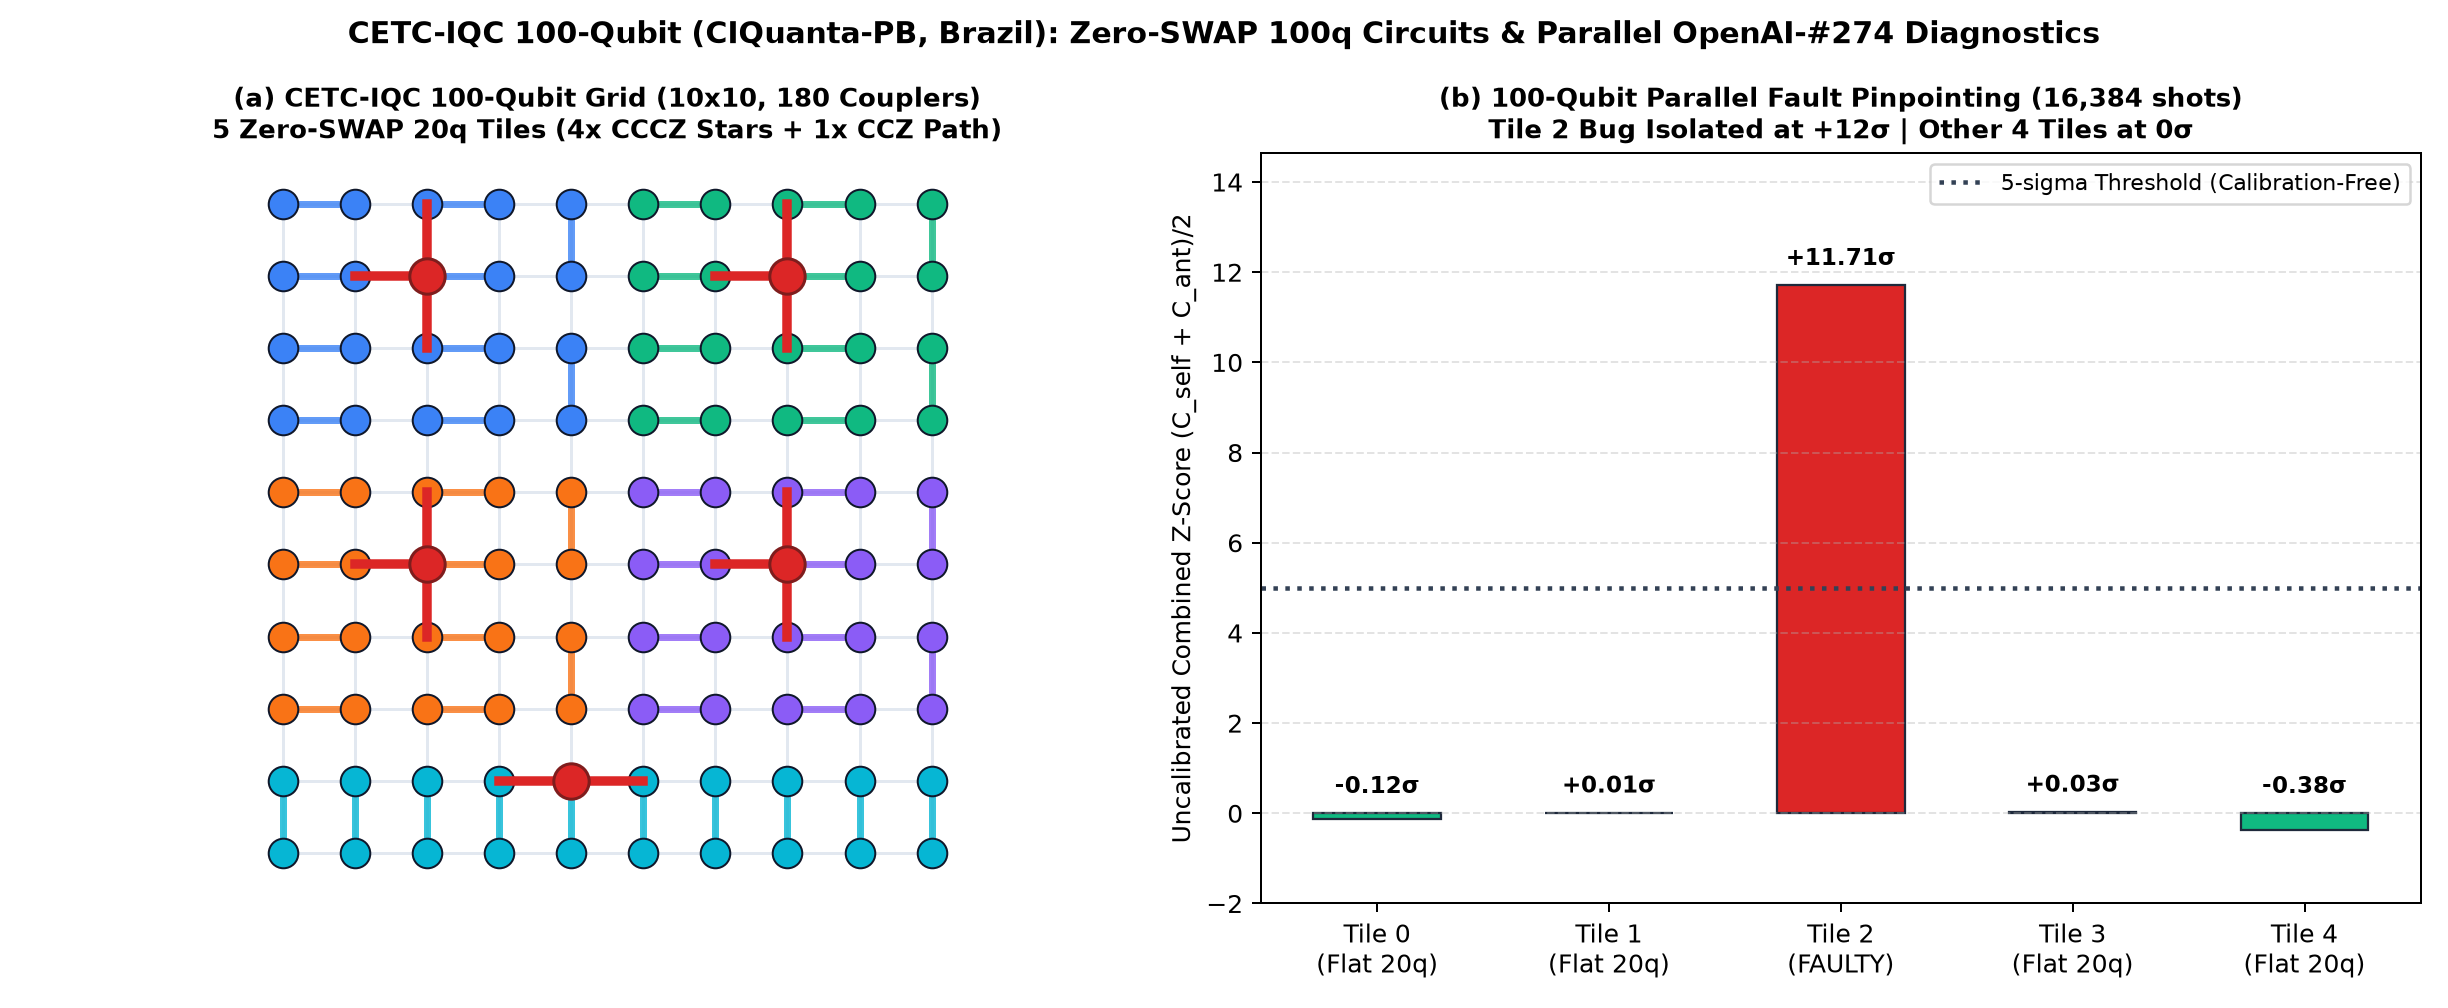
\includegraphics[width=\textwidth]{figures/fig_100q_tiled.png}
\caption{Scalability to a generic $10\times 10$ ($100$-qubit, $180$-coupler) 2D superconducting lattice: (a) exact partition into five zero-SWAP $20$-qubit tiles ($4\times CCCZ$ stars + $1\times CCZ$ path, $0$ SWAPs) and (b) parallel calibration-free fault pinpointing in $16{,}384$ shots isolating a single dropped $CZ$ in Tile~2 at $+11.71\sigma$.}
\label{fig:cetc100}
\end{figure}

\section{Discussion, Reproducibility, and Disclosures}
By uniting classical modular Walsh rigidity (up to $36$ qubits in $128\,\text{GB}$, and $32$ qubits in $4\,\text{GB}$ for $\le 11$ $CCCZ$ gadgets), exact exterior-rank and antipodal obstructions, zero-SWAP Steiner-star compilation, and calibration-free antipodal-felinity diagnostics, we obtain a coherent verification pipeline spanning $20$ to $100$ qubits.

\paragraph{Scope and Limitations.}
Classical modular certification remains $O(n2^n)$ in frequency count and applies specifically to diagonal phase circuits of degree $\le 4$. The $20$- and $100$-qubit hardware benchmarks presented here are Monte Carlo simulations incorporating depolarizing gate errors, coherent over-rotation, and strong asymmetric readout bias on representative 2D lattices; full physical execution on real $20$- and $100$-qubit processors (incorporating live coupler calibration maps, spectator $ZZ$ crosstalk, and $T_1/T_2$ drift) is left as immediate experimental follow-up, for which all physically routed OpenQASM~3.0 circuits and submission scripts are provided.

\paragraph{AI-Assistance Disclosure.}
AI coding and analytical assistants were used to help draft code, execute numerical benchmarks, and format the manuscript; all mathematical statements, unitary audits ($2^{20}$ states), and numerical outputs were independently verified against exact computations.

\begin{thebibliography}{14}
\bibitem{Vono2026Antipodal}
F.~M.~Vono,
\emph{Antipodal Necessity and the Cubic Case of the Homogeneous Rotation-Symmetric Bent Function Conjecture},
Figshare preprint (Version~2), 2026. \url{https://doi.org/10.6084/m9.figshare.34165260.v2}

\bibitem{Vono2026Rigidity}
F.~M.~Vono, A.~O.~N.~de Toledo, and V.~G.~Santos,
\emph{Modular Walsh rigidity for Boolean functions of degree at most four: the uniform $1/2$ bound},
Preprint, 2026. \url{https://doi.org/10.6084/m9.figshare.34963642.v4}

\bibitem{Vono2026H12}
F.~M.~Vono, A.~O.~N.~de Toledo, and V.~G.~Santos,
\emph{Non-Existence of Quartic Homogeneous Rotation-Symmetric Bent Functions in $12$ Variables and the Invariant Half-Space Collapse Theorem},
Preprint, 2026.

\bibitem{Vono2026Exterior}
F.~M.~Vono, A.~O.~N.~de Toledo, and V.~G.~Santos,
\emph{Exterior Rank of a Symbol with the Modulo-Four Obstruction},
Research Note (\texttt{hrsbf-bent-verification}), November 2026.

\bibitem{OpenAI2026QAC0}
OpenAI,
\emph{Product-projection localization and the $\mathrm{QAC}^0$ parity lower bound},
OpenAI Math Release preprint, September 2026 (building on L.~Gretta, M.~Gupta, and M.~R.~Joshi, arXiv:2604.02793, 2026).

\bibitem{Gottesman1999}
D.~Gottesman and I.~L.~Chuang,
\emph{Demonstrating the viability of universal quantum computation using teleportation and single-qubit operations},
Nature \textbf{402}, 390--393 (1999).

\bibitem{Cui2017}
S.~X.~Cui, D.~Gottesman, and A.~Krishna,
\emph{Diagonal gates in the Clifford hierarchy},
Physical Review A \textbf{95}, 012329 (2017).

\bibitem{Rossi2013}
M.~Rossi, M.~Huber, D.~Bru\ss, and C.~Macchiavello,
\emph{Quantum hypergraph states},
New Journal of Physics \textbf{15}, 113022 (2013).

\bibitem{Qu2013}
R.~Qu, J.~Wang, Z.-s.~Li, and Y.-r.~Bao,
\emph{Encoding hypergraphs into quantum states},
Physical Review A \textbf{87}, 022311 (2013).

\bibitem{Gachechiladze2019}
M.~Gachechiladze, O.~G\"uhne, and A.~Miyake,
\emph{Changing the facet of multipartite entanglement with hypergraph states},
Physical Review A \textbf{99}, 052304 (2019).

\bibitem{Rotteler2010}
M.~R\"otteler,
\emph{Quantum algorithms for highly non-linear Boolean functions},
Proc.\ 21st Annual ACM--SIAM Symposium on Discrete Algorithms (SODA), 448--457 (2010).

\bibitem{Leone2022}
L.~Leone, S.~F.~E.~Oliviero, and A.~Hamma,
\emph{Stabilizer R\'enyi Entropy},
Physical Review Letters \textbf{128}, 050402 (2022).

\bibitem{Carlet2021}
C.~Carlet,
\emph{Boolean Functions for Cryptography and Coding Theory},
Cambridge University Press, 2021.
\end{thebibliography}

\end{document}
